This section extends upon the fundamentals mentioned in the general section.

\section{Creating an Account}
The 'General' chapter only briefly mentions creating an account so to make this
section complete as a 'go-to' resource for users it will also be mentioned here
too.

This is where your private communications begin.  Therefore it is important that
this is done correctly otherwise you can't bolster your privacy with our client.

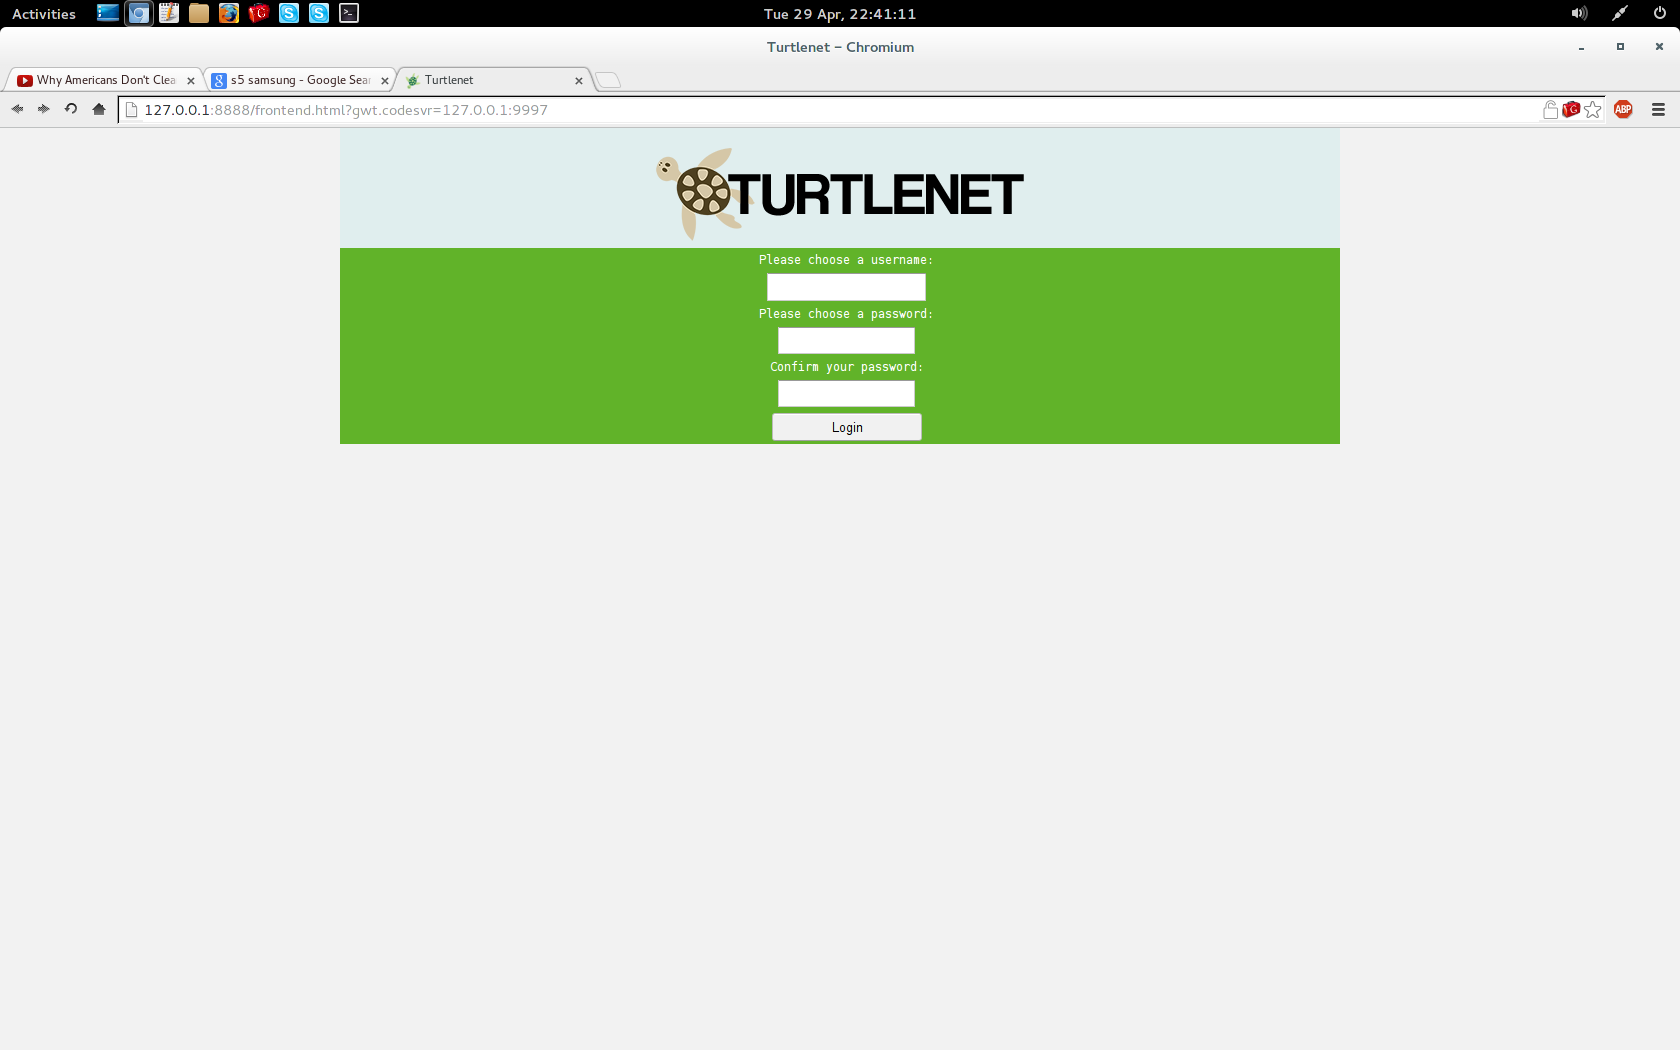
\includegraphics[scale=0.2]{../Screenshots/Screenshot from 2014-04-29 22-41-11}

This image shows the account creation page, which you should see when you run 
the client for the first time on your computer.  From the top there are three
text boxes:
\begin{itemize}
\item a Username box
\item a Password box
\item a Confirmation box
\end{itemize}

You fill in each of the fields with the required information which will be the
following:
\begin{itemize}
\item The Username box should be filled in with your user name.  This is what
      other users would call you when posting messages.  This should be 
      something that represents you, but should not link to you outside of
      Turtlenet.  Simply, your Turtlenet user name should not be the same as
      any other user name you use on the internet.  Can't improve anonymity if
      you use the same name around the internet.
\item The Password is important as it is the only form of validation for logging
      into Turtlenet.  Therefore it should be easy to remember but difficult for
      anyone else to crack.  A good method for coming up with new passwords is
      to use four or five words, like a phrase you use.  An example would be
      'ThisIsTurtlenetzPassword'.  This is better and easier to remember than
      what is usually suggested which is a shorter password with numbers in
      them: 'P@ssw0rd'.  Of course, it depends on who is remembering the
      password so choose your own method if either option mentioned feels
      uncomfortable for you.
\item The Confirmation box is where you type the password you defined in the
      previous box.  Because of this, they should match, and must if the account
      creation is to be successful.  The easiest way of thinking about this box
      is that it is giving you the practice of inputting your password while it
      is still fresh in your mind, to help you remember for later on.
\end{itemize}

By filling in these text boxes with the kind of information mentioned in this
section, you can then click the button underneath these boxes to create your
account.  If successful, the password prompt screen should appear and you can
move onto logging into Turtlenet to begin the communicative fun!

\section{Logging into Turtlenet}
Logging into the Turtlenet client is as simple as using the password that you
had used to create your account, as it is your primary method of informing the
system of who you are.  Please understand that whilst the password is a way of
proving that you are 'you,' other users will not know your password, or even
anything you post until you link them your public key, which will be covered
later in this chapter.

\includegraphics[scale=0.2]{../Screenshots/Screenshot from 2014-04-29 22-24-59}

The screen shot shows the initial page you might see once you have created an
account.  Enter your password into the white text box above the 'Login' button
and if the password is correct, you would have logged in.

\section{Navigating around the Turtlenet client}
Getting around the client's various areas is important in order to make the most
of the functionality provided by Turtlenet.  This is why all of the main
segments are provided as buttons at the top of the interface:

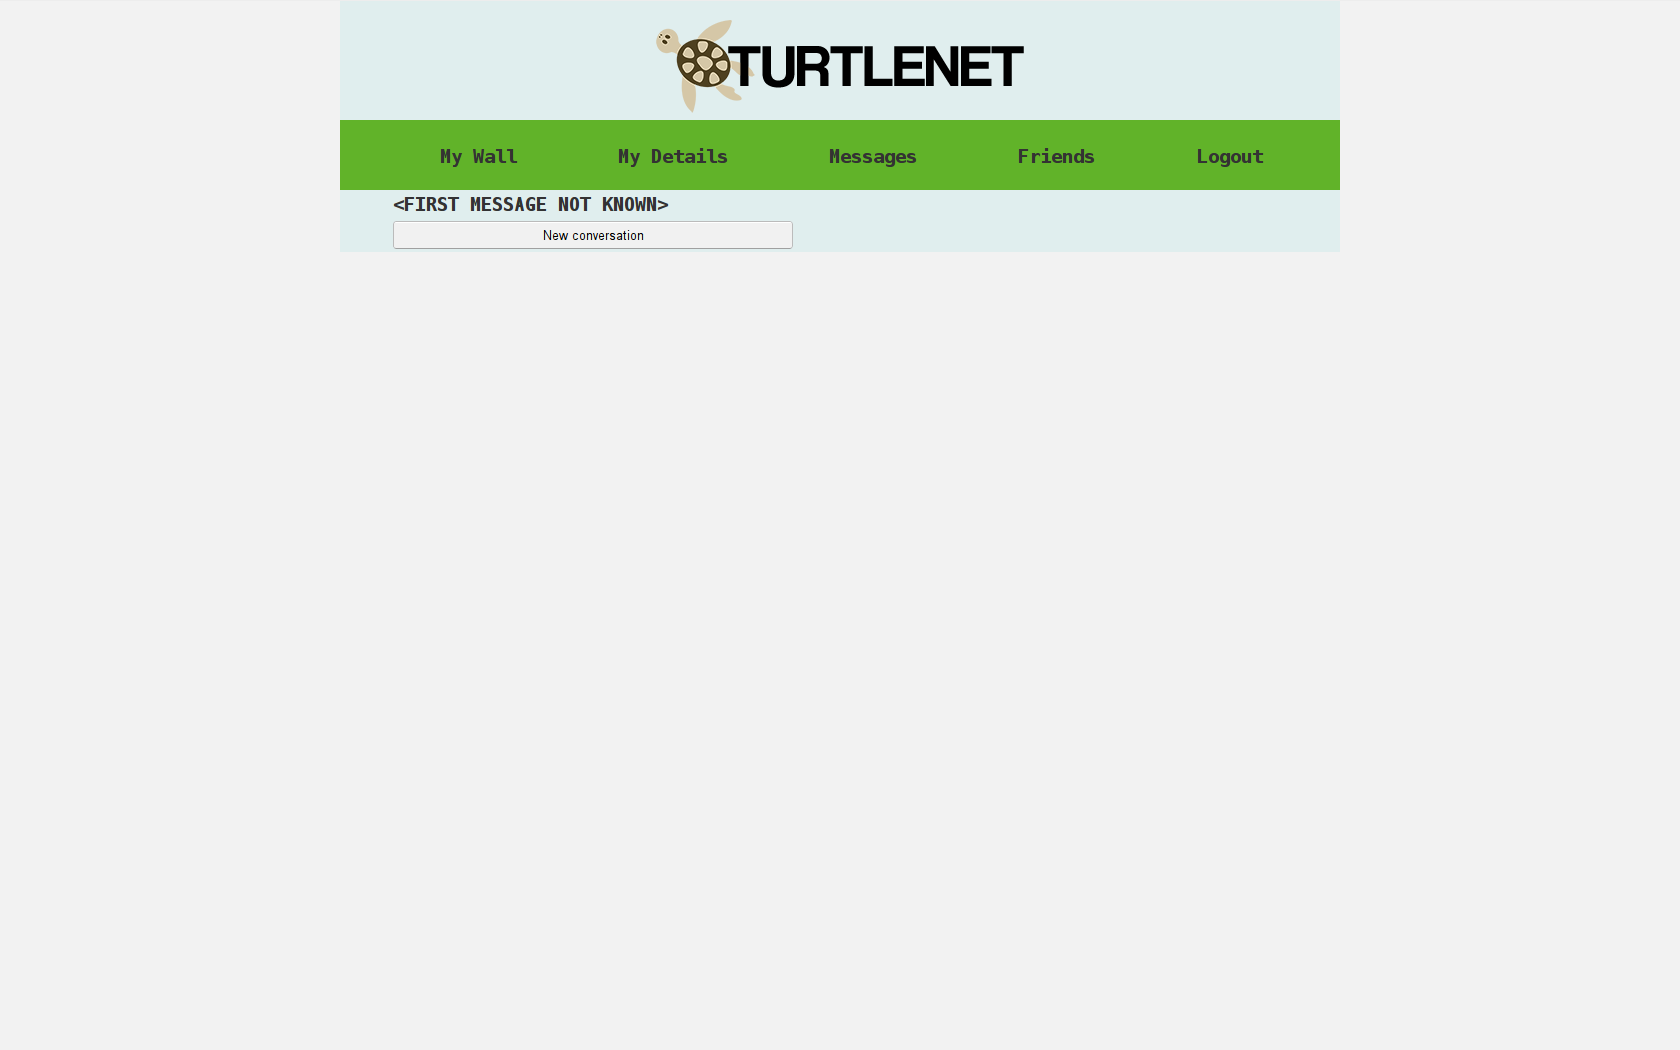
\includegraphics[scale=0.2]{../Screenshots/Screenshot from 2014-04-29 22-31-38}

The image shows that there are several main sections to the client - The wall,
the user's details, messages between the user and other people, friends that the
user has linked with and finally the function to logout.  Click the
corresponding button to get to the area you wish to view.  This chapter will go
through each section from right to left, as it is important to obtain other
users that can read what you post.

\section{Logging out}
